\section{Overview of Market Generator Methods}
\label{sec:model-overview}
  We categorize synthetic financial time series generation methods into
  two main families: classical stochastic (parametric) models, which
  rely on explicit assumptions about the data-generating process, and
  modern deep learning (deep learning) models, which learn complex
  dependencies directly from data without predefined functional forms.
  The following subsections provide a detailed overview of the methods
  included in our benchmark.


  \subsection{Classical Stochastic (Parametric) Methods}
  \label{sub:parametric-methods}
    Parametric models assume a specific functional form for the 
    data generating process, characterised by a finite set of 
    parameters. These models are interpretable and analytically 
    tractable, allowing for closed-form solutions in many cases. 
    However, they may struggle to capture complex stylised facts 
    or high-dimensional dependencies beyond their structural 
    assumptions. Below we outline several widely-used parametric 
    models in financial markets.\\

      \begin{table}[h]
        \centering
        \caption{Common notation and variables.}
        \label{tab:notation}
        \begin{tabular}{ll}
        \toprule
        \textbf{Symbol} & \textbf{Description} \\
        \midrule
        \( S_t \) & Asset price \\
        \( X_t = \ln S_t \) & Log-price \\
        \( r_t = \ln(S_t / S_{t-1}) \) & Log-return \\
        \( \mu \) & Drift \\
        \( \sigma \) & Volatility \\
        \( W_t \) & Standard Brownian motion \\
        \( \Delta t \) & Discrete time step \\
        \bottomrule
        \end{tabular}
      \end{table}
        
        

      \begin{enumerate}[label=\textbf{[A\arabic*]}]
        \item \label{alg:gbm} \textbf{Geometric Brownian Motion 
        (GBM).} 
        The price process follows a continuous-time stochastic 
        process with constant drift and volatility. Model-specific 
        parameters are \(\mu\) and \(\sigma\).
        \begin{equation}
        dS_t = \mu S_t\,dt + \sigma S_t\,dW_t.
        \label{eq:gbm}
        \end{equation}

        \item \label{alg:ou} \textbf{Ornstein–Uhlenbeck (OU).} 
        A mean-reverting Gaussian process for log-prices or 
        spreads. Model-specific parameters are \(\theta>0\) 
        (reversion rate), \(\mu\) (long-term mean), and \(\sigma\) 
        (volatility).
        \begin{equation}
        dX_t = \theta(\mu - X_t)\,dt + \sigma\,dW_t.
        \end{equation}

        \item \label{alg:mjd} \textbf{Merton Jump Diffusion (MJD).} 
        Extends the GBM equation \eqref{eq:gbm} by incorporating 
        normally-distributed jumps. 
        Model-specific parameters are \(\lambda\) (jump intensity), 
        \(\mu_j\) and \(\sigma_j\) (mean and standard deviation of 
        jump sizes).
        \begin{equation}
        \frac{dS_t}{S_t} = \mu\,dt + \sigma\,dW_t + J\,dN_t,\\
        \end{equation}
        where $J \sim \mathcal N(\mu_j, \sigma_j^2),\quad N_t\sim\mathrm{Poisson}(\lambda t)$.


        \item \label{alg:dejd} \textbf{Double-Exponential Jump 
        Diffusion (DEJD).} 
        Another jump-diffusion model with asymmetric double-exponential 
        jump sizes modifying equation \eqref{eq:gbm}. 
        Model-specific parameters are \(p\) 
        (probability of upward jump) and \(\eta_1, \eta_2\) 
        (exponential parameters for upward/downward jumps).
        \begin{align}
          \frac{dS_t}{S_t} &= \mu\,dt + \sigma\,dW_t + Y\,dN_t,\\
          Y &=
          \begin{cases}
          \mathrm{Exp}(\eta_1), &\text{with probability } p,\\[4pt]
          -\mathrm{Exp}(\eta_2), &\text{with probability } 1-p.
          \end{cases} \nonumber
        \end{align}

        \item \label{alg:garch} \textbf{GARCH(1,1).} 
        A discrete-time conditional heteroskedastic model for 
        returns. Model-specific parameters are \(\omega>0,\ 
        \alpha\ge0,\ \beta\ge0\) (GARCH coefficients) and 
        \(\mathcal D\) (innovation distribution, usually standard 
        Normal or Student-t). Captures volatility clustering via 
        time-varying conditional variance.
        \begin{align}
          r_t &= \sigma_t z_t,\quad z_t\sim\mathcal D,\\
          \sigma_t^2 &= \omega + \alpha r_{t-1}^2 + \beta \sigma_{t-1}^2. \nonumber
        \end{align}
      \end{enumerate}


  \subsection{Deep Learning Methods}\label{sub:deep-learning-methods}
    Deep learning models, in this context, refer to generative 
    (often implicit) models that do not assume a fixed parametric 
    form for the underlying data-generating process. Instead, they 
    learn latent structures directly from data through flexible 
    architectures such as neural networks, enabling the modeling 
    of highly nonlinear, high-dimensional, and multi-modal 
    dependencies (e.g., multivariate financial time series with 
    interactions across assets, time horizons, and features). 
    While these models trade off interpretability and analytical 
    tractability, they offer substantially greater expressive 
    power and flexibility. This expressiveness, however, comes at 
    the cost of increased data requirements, more intensive 
    hyperparameter tuning, and higher computational demands. 

    We categorize these approaches into two major families of
    deep generative models, considered in this paper: 
    Generative Adversarial Networks (GANs)
    and Variational Autoencoders (VAEs).
    

  %   \subsubsection{Diffusion Models}
  %     Diffusion models (or score-based generative models) have 
  %     emerged as powerful methods for modeling complex data 
  %     distributions via a forward (noise-adding) process and a 
  %     learned reverse (denoising) process \cite{ho2020denoising}. 
  %     In the forward direction, one gradually corrupts a data sample 
  %     \(x_0\) into noise via a Markov chain:
  %    
  %     \begin{align}
  %       q(x_{1:T}\mid x_0) &= \prod_{t=1}^T q(x_t \mid x_{t-1}), \\
  %       q(x_t \mid x_{t-1}) &= \mathcal{N}\left(x_t; \sqrt{1-\beta_t}\,x_{t-1}, \beta_t I\right). \nonumber
  %     \end{align}
  %    
  %     
  %     The reverse (generative) model is parameterized as
  %     \[
  %       p_\theta(x_{t-1} \mid x_t) = \mathcal{N}\bigl(x_{t-1}; 
  %       \mu_\theta(x_t, t), \Sigma_\theta(x_t, t)\bigr),
  %     \]
  %     where \(\mu_\theta\) and \(\Sigma_\theta\) are often 
  %     expressed via a neural network that estimates the score 
  %     \(\nabla_{\theta} \log p_\theta(x_t)\). A common training 
  %     objective is the simplified denoising score-matching loss:
  %     \[
  %       \mathbb{E}_{t, x_0, \epsilon}\Bigl[ \bigl\| \epsilon - \epsilon_\theta(x_t, t)\bigr\|^2 \Bigr],
  %     \]
  %     where \(x_t = \sqrt{\bar\alpha_t}\,x_0 + \sqrt{1-\bar\alpha_t}\,\epsilon\).
  %     
  %     In finance/time-series, diffusion models have recently been 
  %     adapted to generate synthetic asset paths by converting 
  %     multivariate time series into suitable representations (e.g. 
  %     wavelet-transformed images) and then sampling via reverse 
  %     diffusion \cite{Tanaka25}. For instance, Takahashi and Mizuno 
  %     shows that such an approach can reproduce key statistical 
  %     properties of financial data (e.g.\ volatility clustering, 
  %     tail behavior) \cite{Takahashi24}.  
  %     Another relevant work is "A Financial Time Series Denoiser 
  %     Based on Diffusion Model", which shows how diffusion can help 
  %     improve downstream predictability and reduce noise in 
  %     financial signals \cite{wang24denoiser}.
    \subsubsection{Variational Autoencoders (VAEs)}
    VAEs \cite{kingma2022vae, 
    rezende2014stochastic} are latent-variable generative models 
    that posit a probabilistic encoder \(q_\phi(z \mid x)\) and 
    decoder \(p_\theta(x \mid z)\). One maximizes the evidence 
    lower bound (ELBO):
    \[
    \mathcal{L}_{\text{VAE}} = \mathbb{E}_{q_\phi(z \mid x)}
    \bigl[\log p_\theta(x \mid z)\bigr] - \mathrm{KL}\bigl(
    q_\phi(z \mid x)\,\Vert\,p(z)\bigr).
    \]
    Often one uses a standard Gaussian prior \(p(z) = 
    \mathcal{N}(0, I)\). The encoder–decoder structure allows 
    sampling by first drawing \(z \sim p(z)\), then generating 
    \(x \sim p_\theta(x \mid z)\).
    
    In financial time-series generation, specialized versions such 
    as the Time-Causal VAE (TC-VAE) have been proposed to enforce 
    causality in the encoding/decoding of temporal data. For 
    instance, Acciaio et al.\ (2024) propose TC-VAE, which 
    ensures that generated paths respect temporal causality and 
    show that the model reproduces stylized facts (e.g., heavy 
    tails, volatility clustering) on real markets 
    \cite{acciaio2024vae}. Because VAEs provide a principled 
    latent representation, they are useful in finance to model 
    underlying latent drivers of asset dynamics and to sample 
    coherent trajectories.
    \begin{enumerate}[label=\textbf{[A\arabic*]},resume]
      \item \label{alg:timevae} \textbf{TimeVAE.}
      A time-series specific VAE variant that combines causal
      temporal encoders (e.g., causal convolutions or RNNs) with an
      autoregressive decoder to preserve path coherence. Training
      typically augments the ELBO with prediction or stepwise
      reconstruction losses to improve short- and long-range
      dependencies; TimeVAE is used in our benchmark as a
      dedicated VAE baseline for temporal data \cite{Desai21}.
    \end{enumerate}
    
    \subsubsection{Generative Adversarial Networks (GANs)}
    GANs models approach 
    generation as a two-player game between a generator \(G\) and 
    a discriminator \(D\) \cite{Goodfellow14}. The discriminator 
    is trained to 
    maximize the probability of correctly classifying real data 
    and generated data, with loss
    \[
    L_D = -\mathbb{E}_{x \sim p_{\text{data}}}\bigl[\log D(x)
    \bigr] - \mathbb{E}_{z \sim p(z)}\bigl[\log (1 - D(G(z)))
    \bigr].
    \]
    The generator aims to fool the discriminator and is trained to 
    minimize
    \[
    L_G = -\mathbb{E}_{z \sim p(z)}[\log D(G(z))].
    \]
    Many GAN variants, such as Wasserstein GAN or Least Squares 
    GAN, modify these loss functions to promote more stable 
    training and address issues like mode collapse \cite{Goodfellow14} .
    
    In financial data synthesis, GANs have been widely used to 
    generate realistic synthetic time series. For example, 
    GAN-based financial data generation models (often using WGAN 
    or improvements) show that one can improve the authenticity 
    and predictive ability of generated financial statements or 
    time series \cite{Qi25}. Another example is 
    VRNNGAN, which uses a recurrent VAE as the generator and a 
    recurrent discriminator to capture temporal dependencies in 
    synthetic sequence generation \cite{Lee22}. GANs are 
    relevant in finance because they can capture complex joint 
    distributions and dependencies in multivariate time-series 
    without requiring explicit likelihood models.
    
    \begin{enumerate}[label=\textbf{[A\arabic*]},resume]
      \item \label{alg:quantgan} \textbf{QuantGAN.}
      A GAN variant tailored for financial applications that
      incorporates quantile-aware objectives or conditional
      quantile matching and temporal architectures (e.g.,
      temporal convnets or transformers). QuantGANs aim to better
      capture tail behaviour and risk-sensitive statistics
      (e.g., VaR/CVaR) important for downstream financial tasks
      \cite{Wiese2020}.
    \end{enumerate}
  \subsection{Non-parametric}
  Non-parametric models are generator classes that does not rely
  on probability distribution assumptions or, in the case of Bayesian
  non-parametric models, does not require a specified model parameters.
  Among the simplest but most effective of the non-parametric models are
  the variations of time series block boostrap that, in general, sample
  blocks of time data to preserve temporal dependencies.
  \ref{sub:deep-learning-methods}.
  \begin{enumerate}[label=\textbf{[A\arabic*]}, resume]
        \item \label{alg:blockbootstrap2} \textbf{Block Bootstrap 
        (Resampling Method).} 
        A resampling technique that preserves short-range 
        dependence by sampling contiguous blocks of returns. 
        Although not parametric, it is included here for 
        completeness and baseline comparison.
      \end{enumerate}

      \begin{figure*}[h]
        \centering
        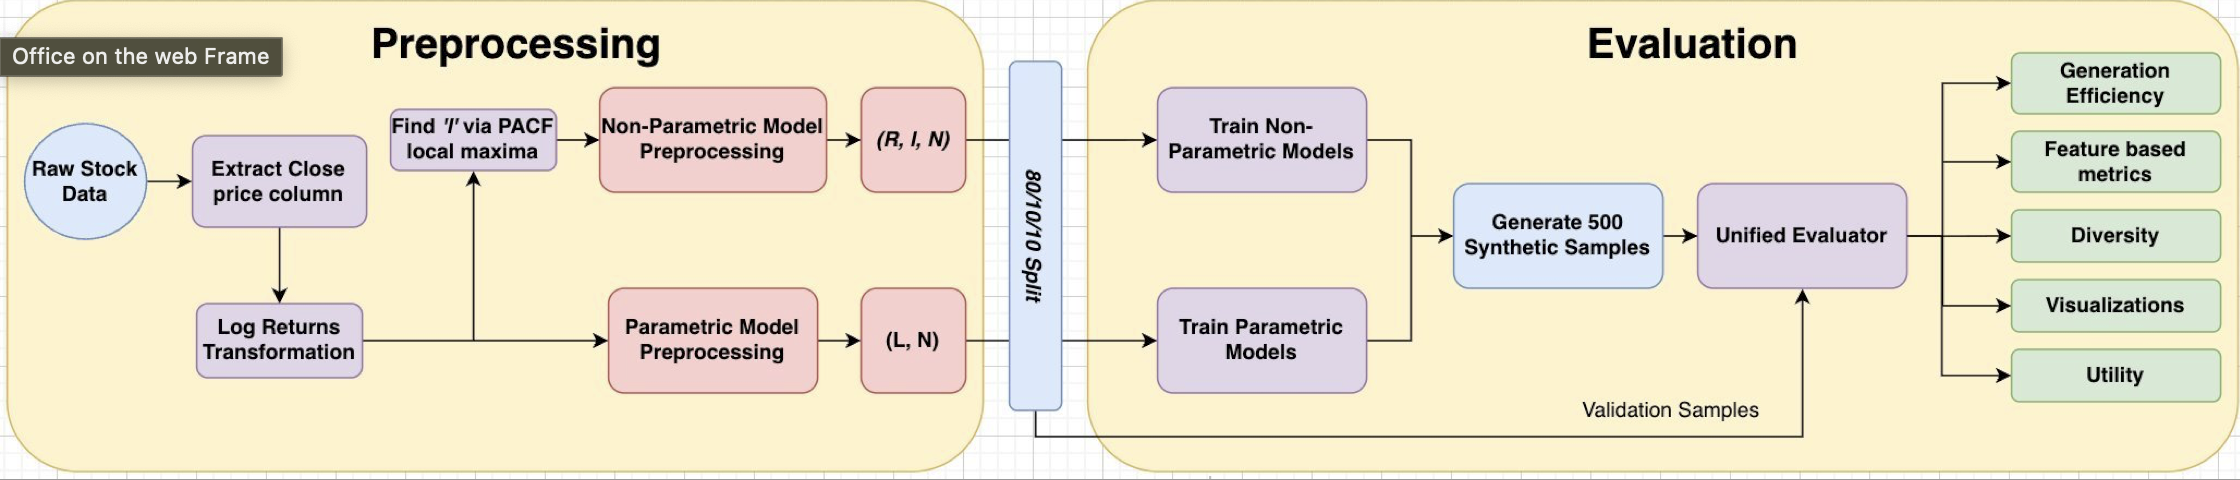
\includegraphics[width=\textwidth,keepaspectratio]{../../results/stonk_bench_architecture.png}
        \caption{Stonk Bench system architecture overview.}
        \Description{Diagram illustrating the complete Stonk Bench pipeline including data preprocessing, model evaluation, and benchmark framework components.}
        \label{fig:stonk_bench_architecture}
      \end{figure*}


